% ATENÇÃO - veja com o seu orientador se você vai ter este capítulo e se este vai ter nome!
\chapter{Metodologia}
\label{cap:metodologia}
Neste capítulo serão discutidos quais foram os passos já tomados e quais serão os passos para a elaboração deste trabalho, desde as pesquisas realizadas para o material bibliográfico, bem como um planejamento das futuras etapas, como pode ser observado na figura \ref{fig:metodologia:etapas} representando as etapas do trabalho. 

\begin{figure}[H]
    \centering
    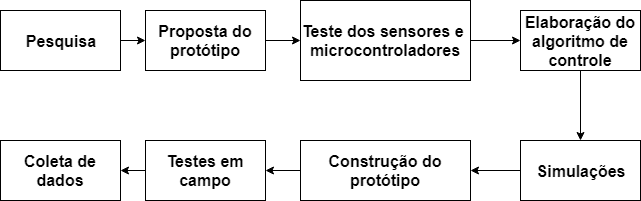
\includegraphics[width=0.8\textwidth]{figuras/metodologia.png}
    \caption{Fluxograma de etapas}
    \label{fig:metodologia:etapas}
\end{figure}

Com o tema definido, foram pesquisados artigos relacionados ao projeto de sistemas fotovoltaicos, o êxodo rural brasileiro, a mecanização do campo e agricultura de precisão, bem como trabalhos científicos com temáticas relacionadas a automação do  maquinário, da construção de protótipos, técnicas utilizadas em relação a movimentação dos veículos. A seguir, foram idealizados os componentes, bem como o chassi do veículo proposto. Durante a busca por trabalhos relacionados, foram usadas diversas bases de dados, tais como  \textit{Institute of Electrical and Electronics Engineers(IEEE) Xplore\footnote{https://ieeexplore.ieee.org/Xplore/home.jsp}, Google Scholar\footnote{https://scholar.google.com.br/}}, dentre outros bancos. 

A elaboração do protótipo foi feita em base das características de conceitos já testados em trabalhos